% \textbf{Social Recommendations:} Software engineering is a social activity~\cite{ahmadi2008survey}, and this principle refers to prioritizing community and social aspects of programming when generating recommendations to developers. In \textit{Nudge}, the authors note ``one of the most effective ways to nudge (for good or evil) is via social influence"~\cite[p.~54]{sunstein2008nudge}. In our results, we found most participants turn to social media and public online resources to learn about new tools. For example, one participant mentioned ``I sorta want to hear about it where I hear about other programming tools. I want to see it on Twitter... It's good when these people have taken the time to talk about it" (P1). Furthermore, Begel et al suggest social media has impacted how software engineers communicate, gain knowledge, and share information~\cite{begel2010social}. An example of social recommendations includes ToolBox, which offers \textit{community sensitive} recommendations for Unix commands based on similar actions by users on a shared network~\cite{ToolBox}. We believe finding ways to integrate social influence and popular opinion into automated recommendations will encourage developer adoption.

% \textbf{User-driven Communication:} User-driven communication refers to the presentation of recommendations to users. Thaler and Sunstein note the importance of communication by writing ``choices can be improved with better and simpler information"~\cite[p.~204]{sunstein2008nudge}. Our survey results show that, while developers had mixed feelings on the conciseness of messages with suggested changes, improving communication during code reviews is the primary advantage of this feature. Additionally, participants in our user study praised the communication in tool recommendations from suggested changes because it can ``comment right here `this fixes your bug', that's nice" (P8). Cerezo and colleagues also suggest that user-driven communication can improve the perception of chatbots as opposed to single-purpose bot-driven techniques~\cite{cerezo2019building}. To improve the effectiveness of automated recommendations to software engineers, we believe providing useful information and comprehensible suggestions will improve the likelihood developers adopt useful tools and practices.


% \textbf{Actionable Recommendation:} Actionability refers to the ease with which users can act on recommendations. In nudge theory, research suggests actionability is a key concept for encouraging humans to make better decisions. A simple nudge is to make target behaviors easy to apply because ``many people will take whatever option requires the least effort, or the path of least resistance"~\cite[p.~85]{sunstein2008nudge}. In our user study, we found developers preferred the suggested changes recommendation because it's ``easier to submit" (P5) and has ``pretty neat integration" (P1). In software engineering research, Heckman and colleagues examined the concept of actionability through static analysis notifications in AAITs (actionable alert identification techniques) to help developers identify and resolve defects in code~\cite{HECKMAN2011363}. We propose making automated development tool recommendations actionable will encourage the adoption from developers.

% \textbf{Receptive Choice Architectures:} Research shows user receptiveness important for making effective recommendations. For example, the \peer study shows that receptiveness significantly impacts the outcome of tool recommendations~\cite{Interactions}. Additionally, Fogg suggests receptive audiences are important for creating persuasive technologies~\cite{fogg2009persuasive}. To leverage nudge theory and choice architecture to improve receptiveness, we suggest emphasizing the locality of recommendations. For contextualizing this concept into design implications, we divide locality into two subcategories: \textit{spatial} and \textit{temporal} locality.

% \textbf{\textit{Spatial:}} Spatial locality refers to the location where recommendations are made. Nudge theory suggests that the location of recommendations matters when encouraging people to adopt useful behaviors. For example, Hanks found that changing the location of vegetables, fruits, etc. in a high school cafeteria increased the purchase and consumption of healthier foods by students~\cite{Hanks2012Lunchroom}. We found that the location of suggested changes was useful for developers in our survey. Furthermore, the fact that our user study participants' interest in adopting tools significantly increased as recommendation systems became more entrenched in the code, i.e. from emails outside of projects to suggested changes on the exact line of code, shows that the location of recommendations matters to developers. Johnson et al. reported that developers felt inconvenienced leaving their normal coding environment to use development tools~\cite{Johnson2013Why}. Similarly, de Alwis and colleagues found that the inability to locate navigation and displays made developers feel disoriented in the Eclipse IDE~\cite{de2006using}. As choice architects for recommendations to developers, researchers and toolsmiths should make automated suggestions to developers in familiar locations to target user receptivity and encourage adoption.

% \textbf{\textit{Temporal:}} Temporal locality references the timing when recommendations are made. In nudge theory, timing also plays a role in impacting human decision-making. For example, changing the timing of fertilizer discounts encouraged farmers in Kenya to make purchases in time to yield higher crops~\cite{duflo2011nudging}. We discovered suggested changes were useful because developers appreciated the timing of recommendations during the code review process.  Research also shows that the timing of recommendations is important in software engineering. For example, changing the time of performing static analysis and distributing tool output encouraged developers at Facebook to fix more reported bugs~\cite{Distefano2019Facebook}. Furthermore, Viriyakattiyaporn and colleagues found that the inability to deliver suggestions in a timely manner discouraged programmers from adopting recommendations to improve code navigation with Spyglass~\cite{viriyakattiyaporn2009challenges}. To incorporate \approaches into recommendations and design receptive choice architectures, we propose developing automated systems to target appropriate times for making suggestions to programmers within their workflow to increase their desire to adopt useful tools and practices.

\section{Approach}

Based on our framework which suggests emphasizing desire, familiarity, social context, and developer workflow to make effective suggestions to software engineers, we propose using digital nudges to send automated recommendations to help improve developer decision-making. This novel approach is more scalable than peer interactions and improves on our \tele by integrating concepts from nudge theory to improve software developer behavior. Thaler and Sunstein present five choice environments when nudges ``are most likely to help and least likely to inflict harm"~\cite[p.~74]{sunstein2008nudge}. We present these scenarios below with examples to describe how they correlate with software engineering and our conceptual framework:

\paragraph{Benefits Now--Costs Later.}

Research shows that humans often participate in activities that provide short term benefits but have long term costs, such as smoking and eating junk food. Nudges can be used to prevent these types of behaviors and raise awareness of the consequences for these activities. For example, nudges to teenagers in Montana were able decrease smoking rates among students~\cite{linkenbach2003most}. In some cases, avoiding developer actions may provide some temporary benefits to development teams. However this can also cause significant problems long term. For example, Xiao and colleagues found that developers reported not adopting security tools to avoid save time and costs on implementing and training for new systems~\cite{Xiao2014Security}. Furthermore, research shows it's better to address issues and adopt useful developer actions early in the development process because the cost to change software increases over time~\cite{SEEconomics}. 

While not adopting new developer actions may provide some benefits such as saving time and money, ignoring useful practices, such as implementing security tools to automatically check for vulnerabilities in code, can ultimately have more serious consequences for development teams over time.  In our preliminary studies, we found cases where users did not desire to adopt tools despite the benefits it would provide. In the \sorry study, we foud developers ignored recommendations because they did not want to adopt new technologies to integrate into their workflow. For example, P11 responded ``Given the number of errors, I think [accepting the recommendation] would cause more harm than good ;)", even though the tool was pointing out errors in the project's code. For the peer interactions study, even though S10 recommends using R because creating a plot will be just two lines of code, S9 replies ``I don't know R" and ignores the suggestion. Using digital nudges to persuade developers to use useful actions can provide them with insight into the long term costs of avoiding adoption.

\paragraph{Degree of Difficulty.}

Research suggests that humans are more likely to need and accept help making selections when faced with solving more difficult and complex decisions. Sunstein and Thaler suggest that ``many problems in life are quite difficult...difficult choices are good candidates for nudges"~\cite[p.~76-77]{sunstein2008nudge}. One example of a hard problem is selecting and paying back student loans. While the process of paying for college used to be simple, the authors note that ``Scholarships and part-time jobs typically do not cover the cost of college [anymore]. So students and their families often turn to student loans to help out...Shopping for a student loan is nearly as complicated as looking for a mortgage"~\cite[p.~141]{sunstein2008nudge}. Bettinger and colleagues implemented the nudge to simplify the Free Application for Federal Student Aid (FAFSA) by incorporating it into the H&R Block\footnote{\url{https://www.hrblock.com}} tax return software to make it easier to compare loan options and increase college enrollment among high school seniors~\cite{bettinger2013fafsa}. Software engineering is another challenging field that has grown more and more complex over time~\cite{SoftwareEatWorld}. Developer decisions require knowledge in a variety of topics such as the technical domain, customers and business, tools and building materials, engineering practices, people and organizations, and more~\cite{GreatSoftwareEngineer}. 

In some cases, we found that developers were unwilling to adopt recommendations for \EP from \tool because they were difficult to integrate. For example, P3 desired the bot to make adoption easier by commenting ``this introduces a bunch of errors, can you check whether they are worth fixing or configure the plugin so as to ignore the false positives?". Participants in the \peer study also avoided using tools that were too difficult, such as when S1 recommends using the Analysis Toolpak\footnote{\url{https://support.office.com/en-us/article/use-the-analysis-toolpak-to-perform-complex-data-analysis-6c67ccf0-f4a9-487c-8dec-bdb5a2cefab6}} in Excel then S2 responding ``This is a little bit weird...No, let's just try to graph this." Using nudges to make effective recommendations can help improve software engineer decision-making by making it simpler to adopt useful behaviors when faced with difficult choices during the development process.

\paragraph{Frequency.}

Decisions and behavioral changes become easier with more opportunities to make similar choices. However, most of the time ``important decisions do not come with many opportunities to practice". But, in this case Thaler and Sunstein suggest ``rare, difficult choices are good candidates for nudges"~\cite[p.~76-77]{sunstein2008nudge}. For example, Madrian and Shea implemented a nudge to persuade employees to enroll in retirement plans by allowing them to opt-out of 401k plans instead of opting in. They discovered this improved money saving behaviors and encouraged more participants to join and more people to join sooner, with 98\% of new employees selecting a plan within 36 months~\cite{madrian2001power}. While software is constantly changing and evolving, developers also face infrequent decisions with significant impact on their products, consumers, and development processes. Examples of these decisions include programming language~\cite{spinellis2006choosing}, licensing~\cite{colazo2009impact}, and architecture~\cite{jansen2005software}. Practitioners must effectively decide on these choices early in development to avoid further costs later on~\cite{SEEconomics}.

In the preliminary work, we also encountered instances of users avoiding adoption because of the severity of the decision to adopt tools. For example, in the \sorry evaluation P14 noted the overhead of incorporating \EP into the build configuration for their specific project saying ``adding the maven-compiler-plugin to a project with packaging=pom with submodules with packaging=archetype is useless". In this case, the developers of the project originally made the decision to implement their continuous integration build with Maven archtypes,\footnote{\url{https://maven.apache.org/archetype/index.html}} which would be difficult to revert and make changes to integrate tools such as \EP. By implementing recommendations as nudges, we believe developers are more likely to improve their behavior when making infrequent decisions about programming activities in their work.

\paragraph{Feedback.} 

While frequency of choices is also impacts decision-making, learning from previous opportunities is also important. Sunstein and Thaler write that people tend to make poor decisions without feedback ``immediate, clear feedback" and ``the best way to help Humans improve their performance is to provide feedback"~\cite[p.~77,~92]{sunstein2008nudge}. For example, a study showed that improving the feedback to households in San Marcos, CA was able to drastically decrease energy usage and improve consumption decisions among users~\cite{schultz2007constructive}. Software engineering research shows feedback is important for developers. For instance, Barik and colleagues examined the impact of compiler error message feedback on how developers resolved problems~\cite{barik2018should} while Johnson and colleagues and found that the primary barrier for static analysis tool adoption for software engineers is result understandability and incomprehensible feedback from these tools~\cite{Johnson2013Why}.

Furthermore, we found that useful feedback is also important within the social context and developer workflow of software engineering. In the \sorry study, many participants complained that our naive bot provided poor feedback by breaking builds for projects and not providing useful information in recommendations to developers. For example, P7 responded `` Also it'd be great to see how ErrorProne would actually help us, e.g. you could attach a report with actual findings in our code base instead of just some generic example". Using digital nudges to improve feedback in automated tool recommendations can help developers make better decisions and adopt useful tools and systems.

\paragraph{Knowing What You Like.} 

Humans rarely select options that are unfamiliar and are prone to make decisions based on previous experiences based on what they already know and like. Nudging is useful for introducing new concepts to people when making decisions. For example, most people order familiar and repeated meals at fast food restaurants based on taste. However, using nudges such as providing information on daily caloric intake recommendations along with calories in food items encouraged consumers to purchase unfamiliar and healthier meals with less calories~\cite{Wisdom2010Healthy}. Many software engineers are comfortable with their current toolsets and environments, which leads to an unwillingness to try new useful development tools and processes. In software engineering, researchers have proposed using history-based recommendation systems use past actions by users to measure desire~\cite{Murphy-Hill2012Fluency}. Additionally, many developers experience \textit{developer inertia} where they are comfortable with their current workflow without tools and avoid adopting new ones.  

A primary result of the \peer study is that familiarity is significant in determining whether users will decide to adopt or ignore tools~\cite{VLHCC}. For example, when L6 asked their partner if they knew R or Python, L5 simply responds ``I don't know Excel" and that was the only software used for the entire study. Similarly, in the \sorry evaluation, we found that in some cases developers weren't familiar with \EP and rejected automated recommendations for the tool. For example, P17 mentioned using other tools such as \textsc{PMD}\footnote{\url{https://pmd.github.io/}} and \textsc{FindBugs}\footnote{\url{http://findbugs.sourceforge.net/}} and stated ``I'm not sure we really need one more analysis tool" in regards to \EP. Nudges such as providing more information to software engineers when recommending unfamiliar development tools can help increase awareness and inform developers of new and better systems for completing programming tasks over their familiar methods.



%\subsection{\TOOL}

%Based on this approach, we plan to implement it in an automated recommender system called, To evaluate approaches for making digital nudges to software engineers for development tool adoption, we developed \TOOL. We aim for researchers to be able to extend this system to recommend useful tools to software engineers. \TOOL~is an automated recommender system designed to suggest software engineering tools to developers on GitHub\footnote{https://github.com}. We target GitHub users because the code hosting and collaboration website has millions of accounts and public repositories, as well as billions of code contributions from developers\footnote{https://octoverse.github.com/}. \TOOL~recommends development tools by integrating with projects' build configuration. With the rise of continuous integration and deployment, many projects implement build systems to automatically compile, test, and release their software more efficiently~\cite{AkondDeployment}. Integrating projects into the build allows developers to easily integrate new tools into their normal software development workflow. An example recommendation prototype from \TOOL is presented in Figure~\ref{fig:approach}.

% \begin{figure*}
% \centering
% 	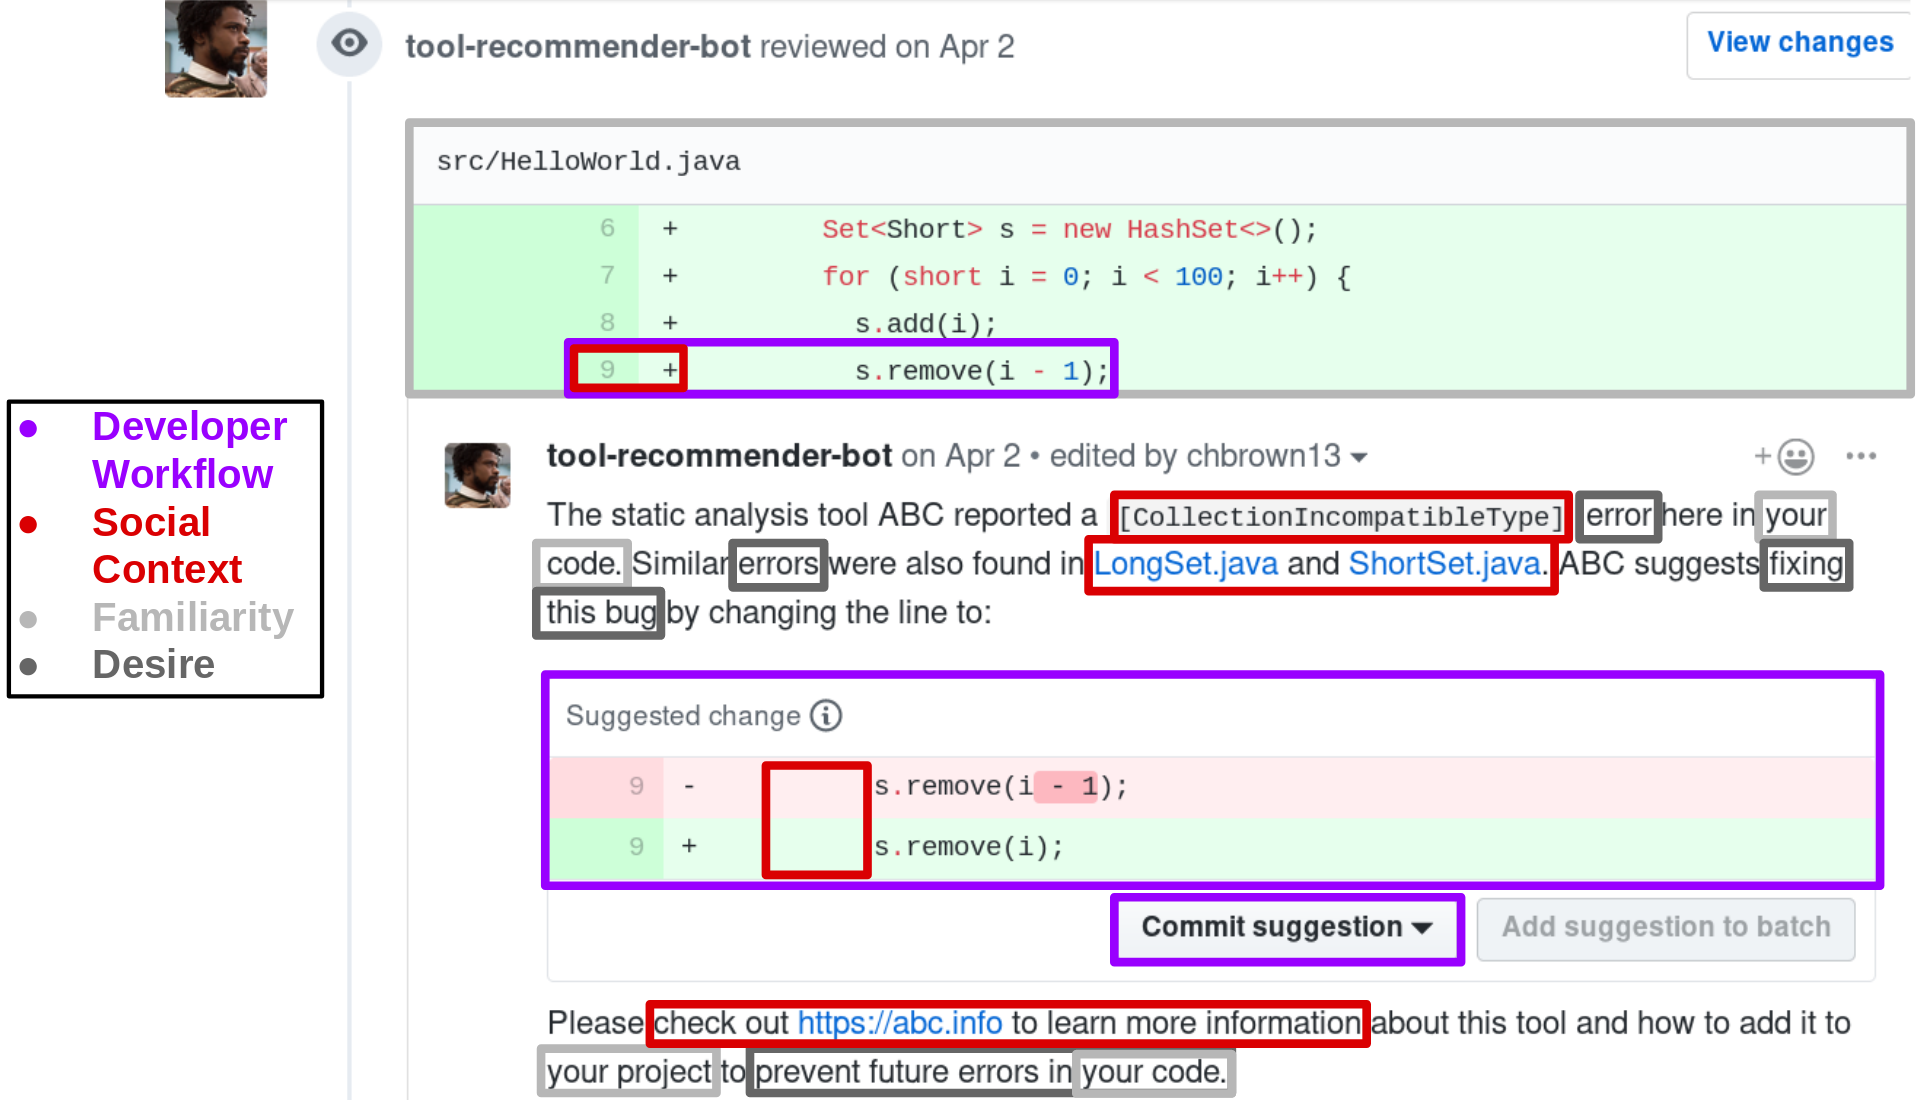
\includegraphics[width=\textwidth]{images/toolapproach.png}
% 	\caption{Prototype implementation of the framework in \TOOL}	
% 	\label{fig:approach} 
% \end{figure*}


% We iteratively modified \TOOL to use different recommendation approaches for nudging developers to adopt different software engineering tools. \TOOL uses a human-presenting GitHub account to recommend tools to developers. Prior work found that bots emulating humans are more effective than bot accounts~\cite{AmongTheMachines}, and we also quickly discovered bot accounts are ineffective for recommendations after our original \TOOL~user\footnote{https://github.com/tool-recommender-bot} was flagged and disabled on GitHub for ``opening multiple unsolicited pull requests in other users' repositories" within a few hours of making recommendations at the beginning of our \tele~study. Our goal is for \TOOL~to integrate numerous recommendation approaches and make software engineering tool recommendations using the most effective nudge type(s) when developers are most receptive to adoption.

%\subsubsection{Spatial.}

%Nudge theory suggests that the placement of options in choice environments, or spatial locality, is an important factor in impacting human behavior and decision-making. For example, the director of food services for a school system with hundreds of thousands of children was able to convince students to eat healthier foods and less junk food by simply changing the arrangement of food choices in the cafeteria, i.e. placing carrots at eye-level instead of French fries. Using this strategy, the director was able to nudge students to adopt better diets and change the consumption of specific food items by up to 25\%~\cite[p.~1]{sunstein2008nudge}. 

%We hypothesize location impacts the effectiveness of recommendations to software engineers. For example, developers are more likely to ignore tool suggestions in emails compared to comments in the code. There are many examples of high spatial locality in software engineering. Most integrated development environments have built-in analyzers that highlight syntax errors at the line of code where developers introduce them. Figure \ref{fig:spatial} shows an example of an error reported by the tool  Pylint\footnote{https://www.pylint.org/}, a static analysis tool for Python. Pylint automatically checks for errors and breaches of coding standards by searching for bad patterns and code smells, and uses the red underline to indicate the exact location of an error in the code base. Furthermore, in prior work we developed a code navigation tool \textsc{Flower}~\cite{Flower}. Our results suggest that participants preferred our \textit{in situ} design and we found that it helped improve their efficiency in completing code searching tasks~\cite{Flower}.

%\subsubsection{Temporal.}

%Research in nudge theory also suggests that timing of recommendations, or temporal locality, plays a role in influencing behavior. One instance of this is the concept of temptation, where Sunstein and Thaler categorize ``hot" and ``cold" states and note that humans are more likely to make certain decisions during hot times~\cite[p.~41]{sunstein2008nudge}. For example, a study found that simply asking people if they intend to purchase a new car within the next six months actually increased purchase rates by 35\%~\cite{morwitz1993intent}. \todo{Better example of timing}

%We examine temporal locality to determine if the timing of tool recommendations to software engineers impacts adoption. \todo{SE example}

%\subsection{Actionability}

%Nudge theory also suggests that actionability, or the ease in which humans can adopt decisions, impacts the choices people make. For instance, a study conducted on Yale seniors found that a lecture on the risks of tetanus, an illness caused by bacteria, was ineffective (3\%) in convincing students to get a shot at the health center. However, providing a campus map to students with the health center circled in the same lecture convinced over nine times more people (28\%) to get the shot~\cite{leventhal1965specificity}. Even though the first group of students knew the location of the health center, adding the map helped students create an actionable plan for getting the shot: allowing them to determine the best route to the health center and how visiting fit in their weekly schedule.

%We believe that actionability is another important factor in the outcome of recommendations to software engineers. \todo{SE example}

% \section{Tools}

This section outlines concepts for tools to develop and existing systems to observe for evaluating our approaches in making effective recommendations to software engineers.

\subsection{\TOOL}

% Prior work indicates \textit{active help systems} are more effective for providing suggestions to software users than passive help systems, which require users to deliberately seek help~\cite{FischerActiveHelp}.

% Research shows using software engineering tools can improve the quality of software and the efficiency of developers, but in reality developers rarely use them.

To evaluate approaches for making digital nudges to software engineers for development tool adoption, we developed \TOOL. We aim for researchers to be able to extend \TOOL to recommend useful tools to software engineers. Our system is designed to target developer receptivity in recommendations: the \textit{desire} of programmers to produce high-quality code and their \textit{familiarity} with a project's code base. \TOOL~is an automated recommender system designed to suggest software engineering tools to developers on GitHub\footnote{https://github.com}. We target GitHub users because the code hosting and collaboration website has millions of accounts and public repositories, as well as billions of code contributions from developers\footnote{https://octoverse.github.com/}. \TOOL~recommends development tools by integrating with projects' build configuration. With the rise of continuous integration and deployment, many projects implement build systems to automatically compile, test, and release their software more efficiently~\cite{AkondDeployment}. Integrating projects into the build allows developers to easily integrate new tools into their normal software development workflow. We iteratively modified \TOOL to use different recommendation approaches for nudging developers to adopt different software engineering tools. \TOOL uses a human-presenting GitHub account to recommend tools to developers. Prior work found that bots emulating humans are more effective than bot accounts~\cite{AmongTheMachines}, and we also quickly discovered bot accounts are ineffective for recommendations after our original \TOOL~user\footnote{https://github.com/tool-recommender-bot} was flagged and disabled on GitHub for ``opening multiple unsolicited pull requests in other users' repositories" within a few hours of making recommendations at the beginning of our \tele~study. Our goal is for \TOOL~to integrate numerous recommendation approaches and make software engineering tool recommendations using the most effective nudge type(s) when developers are most receptive to adoption.

\subsection{\SUGGS}

GitHub recently introduced a new feature that allows developers to suggest a change to a project's code modified by a user.\footnote{https://help.github.com/articles/incorporating-feedback-in-your-pull-request/\#applying-a-suggested-change} Suggestions can be utilized during pull request reviews, allowing reviewers to propose changes at the exact line of code in question and developers to easily accept or reject the change. Code reviews are another example of a software engineering action shown to improve code quality, and early feedback on the suggestion feature shows they are very popular and widely adopted by GitHub users. We plan to evaluate the effectiveness of GitHub suggestions as examples of a \location. These situated nudges already have over 100,000 uses on GitHub projects and developers are ``quick to adopt suggested changes" and integrate this feature into their code review process.\footnote{https://blog.github.com/2018-11-01-suggested-changes-update/} This research aims to examine situated nudges in the context of \SUGGS~to determine if the location of recommendations impacts the effectiveness of adoption for developers.

\subsection{nudge-bot}

